\documentclass[twocolumn,a4j]{jarticle}
\usepackage[dvipdfmx]{graphicx}

\title{DAOの機能改善提案(abstract)}
\author{情報・通信工学科 182C1117 津田 匠貴}
\begin{document}
\maketitle
\section{はじめに}
DAO(Decentralized Autonomous Organization:自立分散型組織)は経済的な共通目的を持った匿名個人らが中央集権的な管理主体を持たず,
特定の国や法定通貨に依存せずに活動を行う組織であり,独自トークンの発行や分散台帳としての記録機能をもつブロックチェーン技術の上に成り立っている.

多くのプロジェクトでは自立分散的に機能するまで株式会社などの中央集権的組織が主体となって運営しているが,彼らによる資金の持ち逃げや売り逃げといった問題が数多く発生しており,問題視されている.
彼らによる不正を防止し,コミュニティによる分散的統治を実現するために,本研究ではEthereumブロックチェーンにおける秘密分散法を用いたメンバーシップの導入と内部告発機能を提案する.
これは不正を行う兆候があるユーザーを検知した場合に内部告発を行い,メンバーの投票による審議を行うことで,不正を防止する流れである.

\section{シャミアの秘密分散法}
シャミアの秘密分散法では,ある秘密を分散情報として管理し,事前に定めた閾値以上の分散情報が集まった場合にのみ復元できるという仕組みである.
各メンバーを$U_1,U_2,...,U_n$とし,素数$p(n<p)$,秘密$s(s∈Z_p)$としたとき,各$U_i$には$d_i∈Z_p$が割り当てられる$(i≠j$のとき,$d_i≠d_j)$.
また,秘密を分散し,配布する役割を担うディーラー$D\notin{{U_1,U_2,...,U_n}}$は秘密$s$から部分情報$s_i$を計算し,$U_i$に配る.
シャミアの秘密分散法における流れは以下のようになる.
\begin{enumerate}
  \item $D$は各$1≦j≦t-1$について,秘密かつ無作為に$a_j∈Z_p$を選び,式(1)のような多項式を定める.
        \begin{equation}
          f(x)=s+a_1x+a_2x^2+...+a_{t-1}x^{t-1}
        \end{equation}

        このとき,秘密$s$について,$s=f(0)$である.
  \item $D$は$U_i$に$s_i=f(d_i)$を送る.
  \item 任意の$t$人のメンバー$U_{i1},U_{i2},...,U_{it}$は式(2)のラグランジュ補間公式を用いることで秘密を復号することができる.
        \begin{equation}
          s=\sum^t_{{k=1}}s_{i_k}\prod_{1≦\ell≦t,\ell≠k}\frac{d_{i_\ell}}{d_{i_\ell}-d_{i_k}}mod p
        \end{equation}

\end{enumerate}

\section{メンバーシップの提案}
DAOにおいて内部告発を実現する場合,以下の二つの条件が矛盾する.
\begin{enumerate}
  \item 全てのメンバーが匿名環境下で活動できる
  \item 不正を行う疑いがあるメンバーを特定する
\end{enumerate}
また,内部告発の対象となる資金の持ち逃げといったインシデントは,その事後に資金の流れを追うことはできても取り戻すことはほぼ不可能であるため,
インシデントが起きる前に不正を防ぐ必要がある.

そのような不正をWeb3上での活動から事前に察知するのは困難だが,Web2上のコミュニケーションツールのチャット内容などから推測できるので,
予めWeb2上のアカウントとWeb3上のアカウントを紐付け,Web2上のアカウントが公開された場合にのみWeb3上のアカウントを特定でき,DAOのメンバーから除外したり資産を凍結するなどの罰則を与える構図を考えた.

このようなスキームであれば,不正を行うリスクが生まれるため,そのような行いを起こそうとするメンバーに対するディセンティブ機構として機能することが期待できる.
また,このスキームにより上述の矛盾を緩和することができる.
\begin{figure}[htbp]
  \begin{center}
    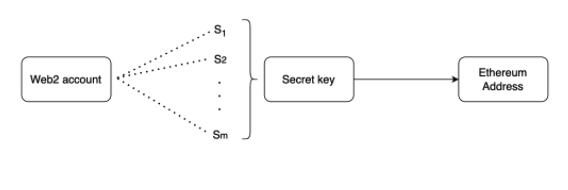
\includegraphics[width=80mm]{account.png}
    \caption{アカウント管理モデル}
  \end{center}
\end{figure}
このモデルはシャミアの秘密分散法を用いており,全てのメンバーは以下の流れに従いアカウントを登録する.
\begin{enumerate}
  \item Ethereum Addressを作成する際に使った秘密鍵を$m$個のsecret shareに分割する
  \item 1つのWeb2 accountにつき,$m$個のsecret shareを紐付けたペアを作る
  \item それぞれのペアは$m$人のメンバーに配られる
\end{enumerate}
これにより,閾値$n$個以上のペアが集まればラグランジュ補間公式より,自身の秘密鍵が復元されEthereum Address上の資産を失うなどのリスクを追うことになる.
このようなリスクを回避する唯一の方法は,自身が内部告発の対象にならないことであり,Web2上で誠実な振る舞いを続け,DAOにとって危害を与えるような言動を慎むことである.

\section{内部告発の流れ}
アカウントを登録した,DAOの内部告発におけるフローチャートは以下のようになる.
\begin{figure}[htbp]
  \begin{center}
    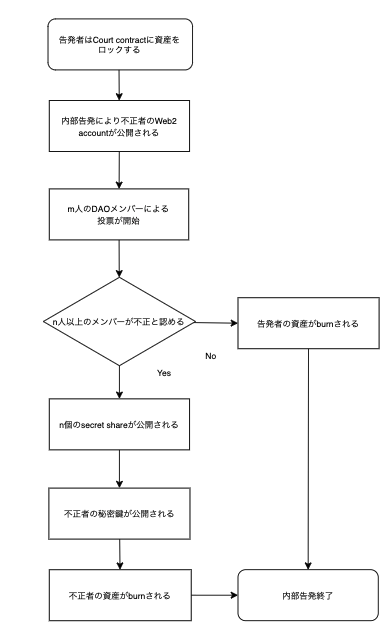
\includegraphics[width=80mm]{flow.png}
    \caption{内部告発の流れ}
  \end{center}
\end{figure}

\section{用語解説}
\begin{itemize}
  \item トークン:ブロックチェーンによって発行,管理される資産や権利のことを指す.
  \item ガバナンストークン:DAOが発行するトークンのことを指す.これは,純粋な資産としての利用のほかに方向性を決める投票権としても利用される.ï
  \item スマートコントラクト:ブロックチェーン上で実行されるプログラムであり,トークンの移動や売買の契約を自動で執行できる.
  \item Web3:ブロックチェーンの登場により唱えられた分散型のwebサービスを総称した概念であり,中央集権的なプラットーフォームに依存しているサービスはWeb2と呼ぶ.
  \item シャミアの秘密分散法:秘密の値をm個のsecret shareに分散しユーザに配布する.閾値以上のsecret shareが再び集まれば秘密の値を復元できる.
  \item ゼロ知識証明:ある命題の答えを知っていることを,その答え自体を示さずに証明する方法
\end{itemize}


\begin{thebibliography}{99}
  \bibitem{sincho} 神宮武志,古田英之,岩村惠市,"秘密分散法における検証可能な分散情報の更新手法",2014
\end{thebibliography}

\end{document}
